    \documentclass[unknownkeysallowed]{beamer}

    \usepackage{beamerthemesplit}
	\usepackage{colortbl}

\usetheme{Warsaw}
\title[Le equazioni di Eulero Poincare']{ Teoria dei gruppi di Lie \\ approccio gruppale alla meccanica classica.}
\author{AMM}
\institute{Universita' Milano Bicocca}
\date{30 novembre, 2010}

\usepackage{amsmath}
\usepackage{amsfonts}
\usepackage[mathscr]{eucal} 
\usepackage[utf8]{inputenc}
\usepackage[italian]{babel}
\usepackage{listings}
\usepackage{textcomp}
\usepackage{graphicx}
\usepackage{subfigure}
\usepackage{caption}
\usepackage{latexsym}
\usepackage{epstopdf}
\usepackage{eepic,epic,eepicemu}
\usepackage{color}
\usepackage{soul}
   
\begin{document}

\begin{frame}
\titlepage
\end{frame}

\begin{frame}{Articolo di Poincarè}
\begin{columns}
\begin{column}[l]{.5\textwidth}
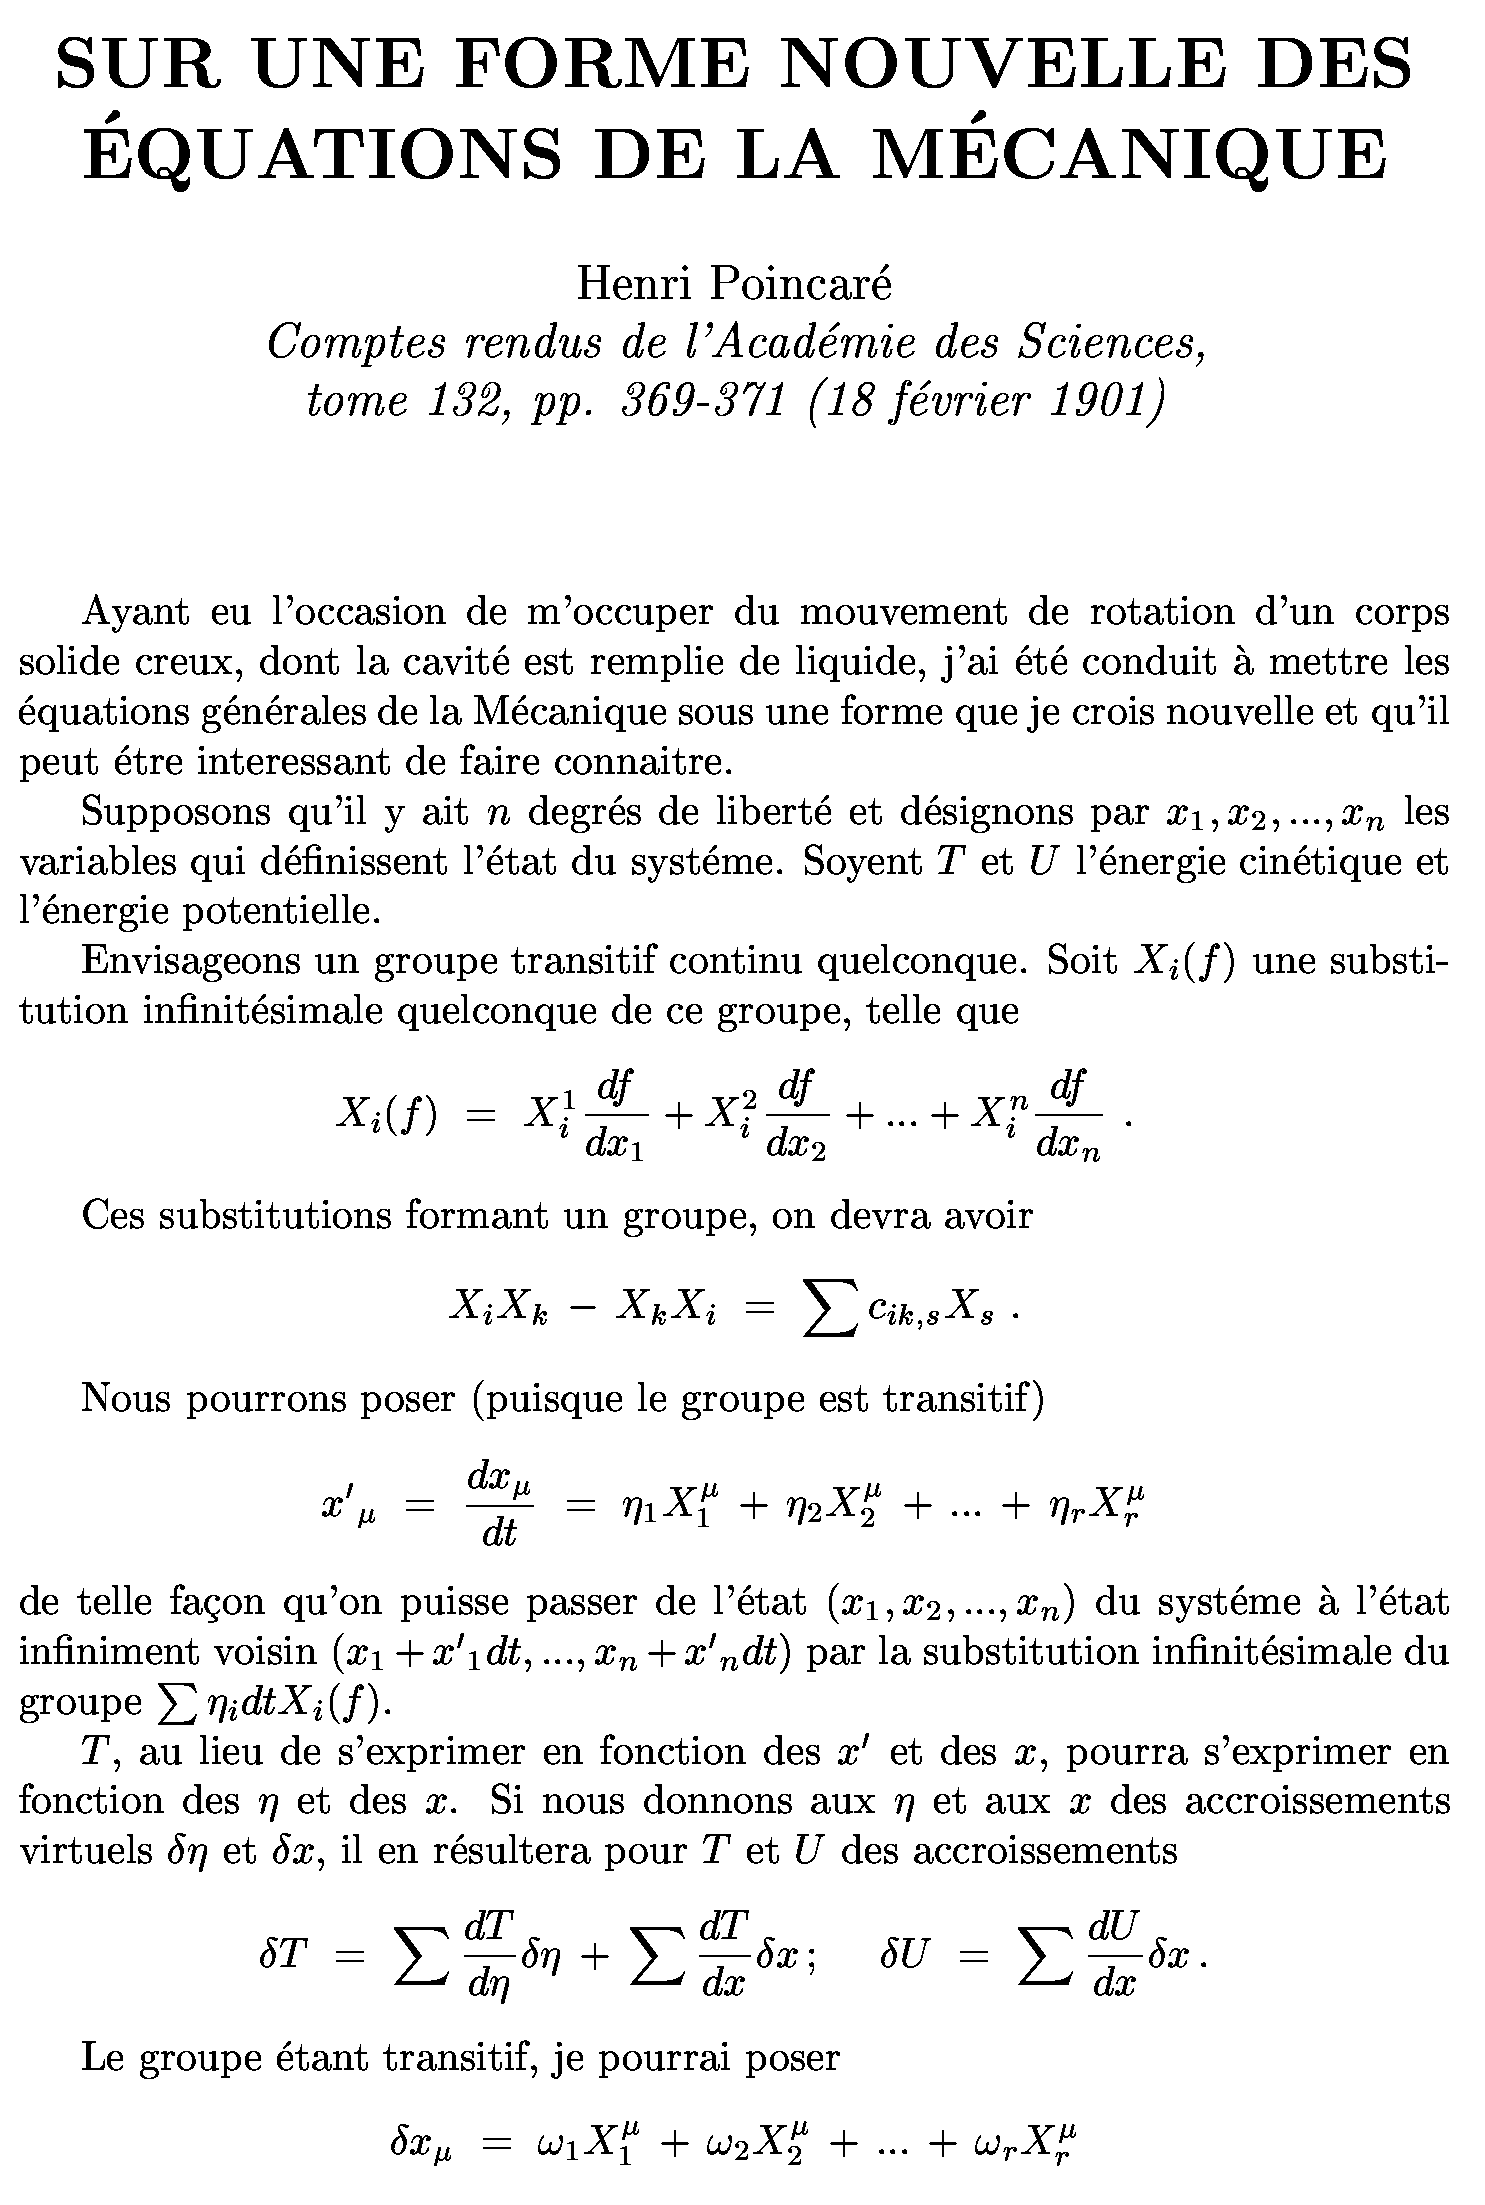
\includegraphics[height=8cm]{Articolo/poincare_epag1}
\end{column}
\begin{column}[r]{.5\textwidth}
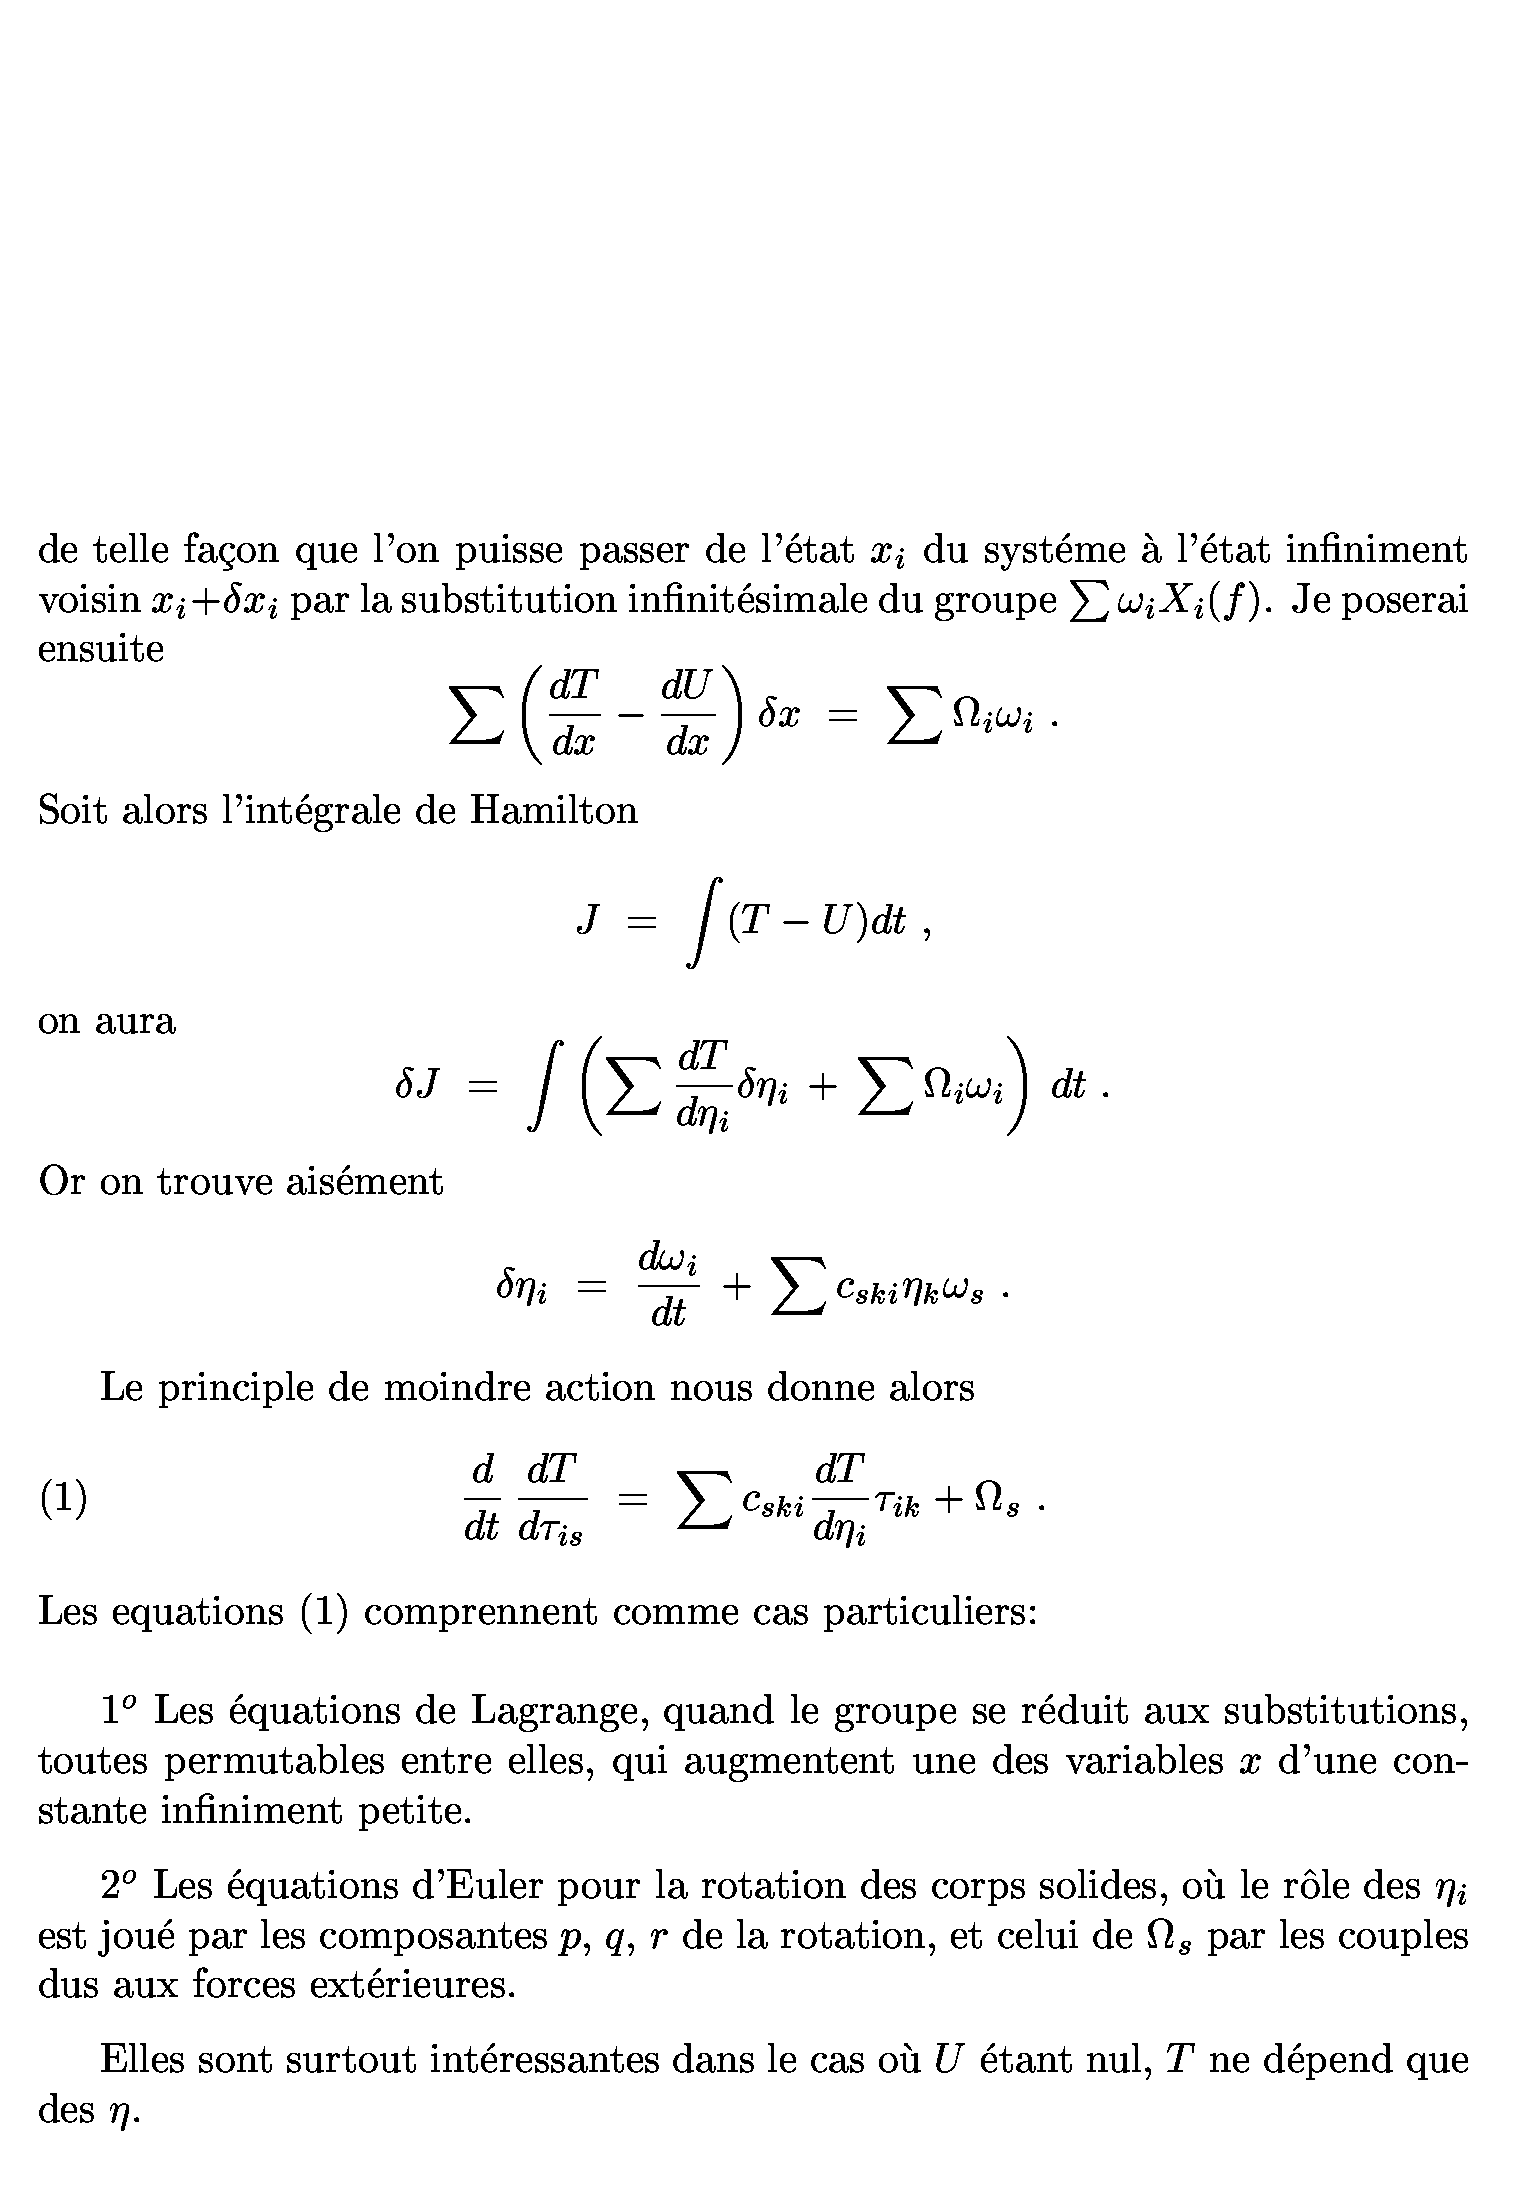
\includegraphics[height=8cm]{Articolo/poincare_epag2}
\end{column}
\end{columns}
\end{frame}

\begin{frame}{Articolo di Poincarè}
Nell'articolo appaiano per la prima volta le equazioni di Eulero Poincarè 
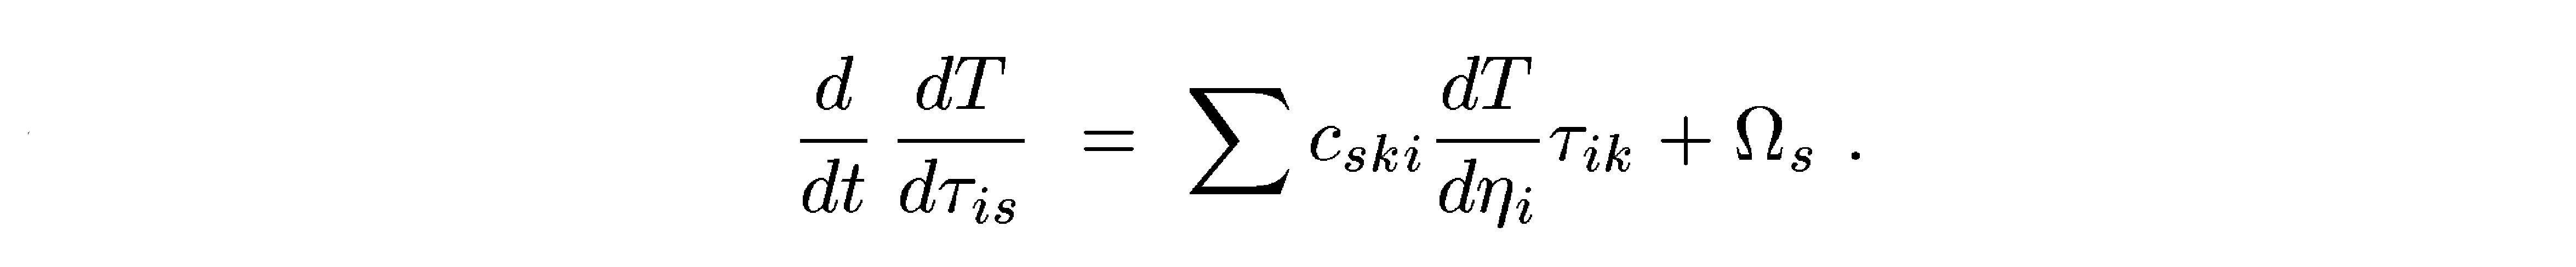
\includegraphics[height=1cm]{Articolo/EP}

%con esplicito riferimento al moto dei corpo rigidi.
\vfill

Nelle equazioni del moto entra esplicitamente la struttura gruppale dello spazio di configurazione.
\\ Compaiono al loro interno i coefficienti $C_{\, s\, k \, i} $, \underline{Costanti di Struttura} del gruppo.


%Nelle parole di Poincarè si intravadendono tutti i presupposti per la derivazione di queste equazioni:
 %\begin{quote}
 %\large
 %$[...]$ J'ai ètè conduit à mettre les \alt<1>{\color{black}équations générales de la Mécanique}{\color{red} équations générales de la Mécanique} 
%\color{black} sous une 
%\alt<1,2>{\color{black} forme }{\color{blue} forme }\color{black} que je crois %\alt<1,2>{\color{black} nouvelle }{\color{blue} nouvelle }\color{black}.
%\\ $[...]$ Envisageons un \alt<1,2,3>{\color{black} groupe }{\color{green} groupe }\color{black} transitif continu \alt<1,2,3,4>{\color{black} quelconque }{\color{black} quelconque }\color{black}. \end{quote}

\end{frame}


\begin{frame}{Struttura Della Tesi}
\begin{columns}[c] % the "c" option specifies center vertical alignment
\column{.5\textwidth} % column designated by a command

\begin{block}{Elementi di Teoria dei Gruppi di Lie}
%\uncover<1->{\begin{itemize} \item Traslazioni \item Algebre \item Azioni \item Gruppi di Matrici \end{itemize}}
\end{block}
\vfill
\phantom{1}

\phantom{1}

\phantom{1}

\phantom{1}

\phantom{1}

\phantom{1}

\phantom{1}

\uncover<3->
{\begin{alertblock}{Equazioni di Eulero e E-P}
%\begin{itemize} \item Derivazione vettoriale delle equazioni di Eulero per il C.R \item Interpretazione algebrica delle equazioni di Eulero \item EQUAZIONI EULERO POINCARÈ \end{itemize}
\end{alertblock}}

\column{.5\textwidth}
\uncover<2->{
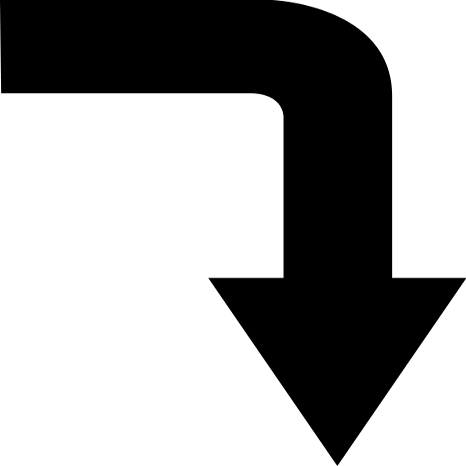
\includegraphics[width=1.5cm,keepaspectratio]{Fig/freccia_1.png}
}
\begin{center}
\uncover<2->
{\begin{exampleblock}{Il gruppo delle Rotazioni e La cinematica del Corpo Rigido}
%\begin{itemize} \item Rappresentazioni \item Strutture \item Lo spazio di configurazione del corpo rigido \end{itemize}
\end{exampleblock}}
\end{center}
\uncover<3->{
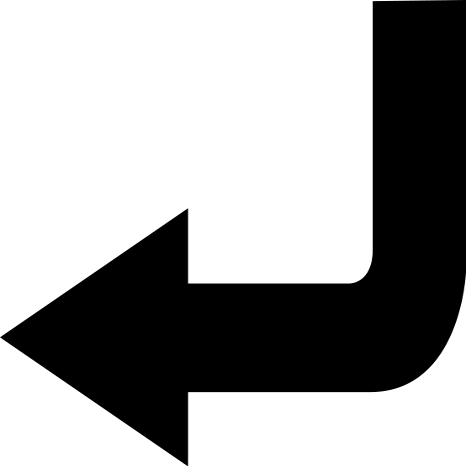
\includegraphics[width=1.5cm,keepaspectratio]{Fig/freccia_2.png}}


\end{columns}
\end{frame}


\begin{frame}{Algebre e Gruppi di Lie}
Temi affrontati:
\begin{itemize}
\item Definizione astratta di Gruppo di Lie.
\item Definizione delle strutture invarianti (traslazioni, campi e 1-forme) e loro proprietà.
%\pause
\item Algebra di un gruppo di Lie.
%\pause
%\item Strutture di collegamento tra l'algebra e il gruppo.
%\pause
\item Rappresentazioni e azioni del gruppo su se stesso (azione aggiunta e coaggiunta).
%\pause
\item Realizzazione delle strutture presentate nel caso di gruppi di matrici.
\end{itemize}
\end{frame}

\begin{frame}{Il gruppo delle Rotazioni}
Temi affrontati:
\begin{itemize}
\item Presentazione del gruppo $\mathscr{R}$ delle rotazioni in astratto.
%\pause
\item Parametrizzazione del gruppo e identificazione con $SO(3)$.
%\pause
\item Identificazione di $SO(3)$ con lo spazio di configurazione del C.R. con punto fisso.
%\pause
\item Studio delle strutture di $SO(3)$.
\end{itemize}
\end{frame}


\begin{frame}{Equazioni di \emph{Eulero} e \emph{E-P}}
Temi affrontati:
\begin{itemize}
\item Presentazione delle equazioni di Eulero e loro interpretazione algebrica.
%\pause
\item Introduzione dell'\emph{Equazione Centrale della dinamica}.
%\pause
\item Studio dell'equazione centrale nell'ipotesi che lo spazio di configurazione possieda la struttura di gruppo di Lie.
%\pause
\end{itemize} \end{frame}

\frame{\frametitle{Obiettivo}
Interpretazione dei risultati orginali di Poincarè in un linguaggio moderno.
\vfill
\begin{tabular}{l c c}
\emph{équations générales} & $ \Longrightarrow $ & Equazione Centrale della Dinamica \\
\emph{\small group transitif continu} & $ \Longrightarrow $ & Spazio di configurazione $\equiv$  Gruppo di Lie \\
\emph{forme nouvelle} & $ \Longrightarrow $ & Equazioni EP \pause \\
\end{tabular}
\vfill

\begin{exampleblock}{\centering TESI}
Le Equazioni EP sono la proiezione dell' Equazione Centrale sulla base delle 1-forme invarianti.
\end{exampleblock}}


\begin{frame}{Formulazione Lagrangiana Classica}\label{1 Formulazione Lagrangiana Classica}
Concetti chiave della formulazione lagrangiana della meccanica classica:
\begin{itemize}
\uncover<2->{\item Lo spazio di configurazione di un sistema meccanico \textbf{Q} è una varietà differenziale.}
\uncover<3->{\item Il fibrato tangente allo spazio di configurazione, \textbf{TQ}, congloba in se tutta la cinematica del sistema concessa dai suoi vincoli.}
\uncover<4->{\item La dinamica di un generico sistema conservativo è tutta racchiusa in una funzione
$$L : TQ \rightarrow R $$
detta \textbf{lagrangiana}.}
\end{itemize}

%\uncover<5->{\begin{block}{Principio Primo}
%Siano $( q^{i}, \dot{q}^{j})$ un sistema di coordinate sulla varietà Q.I moti \emph{naturali} effettivamente compiuti dal sistema durante la sua evoluzione temporale sono le curve $\gamma \in TQ$ tali per cui la valutazione della funzione lagrangiana su di esse soddisfa l'equazione:
%$$     \frac{d}{dt}\left(\frac{\partial L}{\partial \dot{q}^\lambda}\right) -\frac{\partial L}{\partial q^\lambda}=0$$}
%\end{block}

\end{frame}

\begin{frame}{Verso l'equazione Centrale}\label{2 verso L'equazione Centrale}
È possibile definire due forme differenziali:
%,1-forme sul fibrato tangente $TQ$
:

\begin{itemize}
\uncover<2->{\item La 1-forma \textbf{Lavoro di Lagrange}:
$$l_{\,L}\, = \vec{F}\cdot \textrm{d}P + \textrm{d}T = \, \textrm{d}L $$
}
\uncover<3->{\item La 1-forma \textbf{Azione di Maupertuis}
$$a_{\,M}\, = \vec{p}\cdot \textrm{d}P =  p_{k}\: \textrm{d} x^{k} = \frac{\partial L}{\partial \dot{x}^{\,k}} \, \textrm{d} x^{k} $$
%\dfrac{\partial L}{\partial x^{i}} \cdot
}
\end{itemize}

\uncover<4->{
\begin{block}{Principio dell'equazione centrale}
I moti \emph{naturali} avvegono sempre in modo da verificare in ogni punto l'equazione

\begin{displaymath}
\dfrac{\textrm{d}}{\textrm{d}t}a_{M} = l_{L}
\end{displaymath}

Detta \textbf{Equazione Centrale della Dinamica}.
\end{block}
}
\end{frame}

\begin{frame}{\emph{Esempio}: Equazioni di Lagrange }\label{3 l'Equazione Centrale Della Dinamica}
Nelle coordinate $(q^{k}, \, \dot{q}^{k})$ e sulla base $(\textrm{d} q_{\,k}\, , \textrm{d} \dot{q_{\,k}})$ risulta:
\begin{displaymath}
a_{M} = p_{k} ( q, \dot{q}) \textrm{d} q^{k}
\qquad
l_{L} = \textrm{d} L( q, \dot{q}) = \dfrac{\partial L}{\partial q^{k}}\, \textrm{d} q^{k} + \dfrac{\partial L}{\partial \dot{q}^{k}}\, \textrm{d} \dot{q}^{k} 
\end{displaymath}
\uncover<2->{L'equazione centrale assuma la forma:
\begin{displaymath}
\dot{p_{\,k}} \textrm{d} q_{\,k} + p_{\,k} \textrm{d} \dot{q_{\,k}} = \dfrac{\partial L}{\partial q^{k}}\, \textrm{d} q^{k} + \dfrac{\partial L}{\partial \dot{q}^{k}}\, \textrm{d} \dot{q}^{k} 
\end{displaymath}}%\end{frame}%\begin{frame}{Equazione centrale $\Rightarrow$ Equazione Lagrange (2)}
\uncover<3->{Uguagliando i coefficienti delle 1- forme :
\begin{displaymath}\begin{split}
\textrm{d} \dot{q_{k}} &: \qquad p_{\,k} = \dfrac{\partial L}{\partial \dot{q}_{\,k}}\\
\textrm{d} q_{k} &: \qquad \dot{p}_{\,k} =  \dfrac{\partial L}{\partial q_{\,k}}\\
\end{split}\end{displaymath}}
\uncover<4->{
Eliminando i momenti canonici :
\begin{alertblock}{\centering \textbf{equazioni Eulero-Lagrange}}
\begin{displaymath}
\dfrac{\textrm{d}}{\textrm{d}t} \dfrac{\partial L}{\partial \dot{q_{\,k}} } - \dfrac{\partial L}{\partial q_{\,k} } = 0
\end{displaymath}
\end{alertblock}
}
\end{frame}


\begin{frame}{Coordinate sul fibrato tangente di un gruppo di Lie}\label{4 Dalle coordinate Lagrangiane alle coordinate Euleriane}

Costruzione del sistema di coordinate dei campi invarianti: \vfill
\begin{itemize}
\uncover<2->{\item Si fissa un sistema di coordinate $x^{i}$ arbitrario sulla varietà $G$.
}
\uncover<2->{\item Si fissa una base $\xi_{i}$ di vettori sull'algebra $\mathfrak{g}$ del gruppo.
}
\uncover<3->{\item Ad una base di vettori nell'algebra si associa una base $ X_{i}$ di campi invarianti ( a destra o a sinistra).
}
\uncover<3->{\item Ad una base di campi invarianti si associa la base di 1-forme invarianti (a destra o a sinistra) $\epsilon^{\, j}$ tale che $ \epsilon^{\, j} ( X_{i} ) = \delta ^{j}_{\, i}$.
}

\uncover<4->{\item Sfruttando le 1-forme invarianti è possibile associare le componenti di un generico vettore tangente sulla base invariante. Si definiscono le \emph{quasivelocità} come: $ v^a = \epsilon^a (v)$.
}

\end{itemize}


\uncover<5->{\begin{alertblock}{La 2-npla di funzioni $(x^i, v^a)$ costituisce un sistema di coordinate su $TG$.}
\end{alertblock}}
\end{frame}

\begin{frame}{Decomposizione dell'equazione Centrale}\label{5 Decomposizione dell'equazione centrale}
Alle coordinate appena scelte si associa la base non naturale delle 1-forme $(\epsilon^{a} , \, \textrm{d}v^{b}) $.
\vfill

\uncover<2->{Decomponendo le 1-forme su questa base:
\begin{displaymath}
a_{M} = p_{\, a} \epsilon^{a}
\qquad
l_{L} = \textrm{d}L ( x,\,v )
\end{displaymath}
L'equazione centrale diventa:
\begin{displaymath}
\dot{p}_{\,a} \, \epsilon^{a} + p_{a} \dfrac{\textrm{d} \, \epsilon ^{a}}{\textrm{d} t} = \dfrac{\partial L}{\partial x^{i}} \textrm{d}x^{i} + \dfrac{\partial L}{\partial v^{a}} \textrm{d}v^{a}
\end{displaymath}}
%\\Che contiene 1-forme non appartenenti alla base scelta.
\vfill
\begin{center}
\uncover<3->{
Resta da capire come si calcola: $$\dfrac{\textrm{d} \, \epsilon ^{a}}{\textrm{d} t}$$
Serve l'\emph{identità di Hamel-Boltzman}.
%Restano quindi due questioni da risolvere: 
}
%\begin{enumerate}[<3-| alert@+>]
%\item  Calcolare la derivata temporale delle 1-forme invarianti.
%\item  Decomporre la 1-forma $\textrm{d}x^{\, i}$ sulla base prescelta.
%\end{enumerate}
\end{center}
\end{frame}


%\begin{frame}{Cambio di coordinate sul fibrato tangente}\label{6 Cambio di coordinate sul fibrato tangente}
%Data la matrice $A_{i, \, j}$ delle componenti delle 1-forme invarianti sulla base naturale risulta:
%\vfill \begin{center}

%\begin{tabular}{l c}
%$ \epsilon^{a} = A^{a}_{\: j} \, \textrm{d}x^{j} $ & $ \textrm{d} x^{j} = \bigr( A^{-1}\bigr)^{j}_{\: a}\,  \epsilon^{a} $ \\ & \\ & \\
%$v^{a} = \epsilon^{a}(v) = A^{a}_{\:j}\, \textrm{d}x^{j}(v) = A^{a}_{\:j} \, \dot{x}^{j} $ \quad & $  \dot{x}^{j} = \bigr( A^{-1}\bigr)^{j}_{\: a}\, v^{a} $
%\end{tabular}
%\end{center}
%\end{frame}

\begin{frame}{Identità di Hamel Boltzman}


\begin{alertblock}{Tesi}
Vale l'equazione: 
\begin{displaymath}
\dfrac{\textrm{d}\epsilon^{a}}{\textrm{d}t} = \textrm{d}v^{a} - C^{a}_{\: b \, c}v^{c}\,\epsilon^{b}
\end{displaymath}\end{alertblock}

\vfill
\uncover<2->{
Per dimostrarla ci si avvale fondamentalmente di due ipotesi:%}
\begin{itemize}
%\uncover<3->{
\item É nota la matrice $A_{i, \, j}$ di cambio di base tra la base naturale e la base delle 1-forme invarianti.%}
%\uncover<4->{
\item È valida la \emph{Regola di scambio} \begin{displaymath}
\dfrac{\textrm{d}}{\textrm{d}t} \textrm{d}x_{\,k} = \textrm{d}\dot{x_{\,k}}
\end{displaymath}
}
 
\end{itemize}

%\vfill \uncover<5->{Cenni della dimostrazione:} 
%\begin{itemize}
%\uncover<6->{\item si decompone la 1-forma $\epsilon$ sulla base naturale.}
%\uncover<7->{\item si calcola la derivata temporale sfruttando la regola di scambio.}
%\uncover<8->{\item si ritorna alla decomposizione sulla base $( \epsilon^{a}\, , \textrm{d} v^{b} ) $ sfruttando l'inverso della equazioni di cambio di base e le loro conseguenze differenziali.}
%\end{itemize}
\end{frame}


\begin{frame}{Equazioni di Eulero Poincarè}
È possibile ora decomporre l'equazione centrale sulla base $ (\epsilon^{a}, \textrm{d} v^{a})$.

\begin{displaymath}
(\dot{p}_{a} - C^{b}_{\: a, c} \, p_{\,b} \, v^{c}) \epsilon^{a} + p_{\,a}\, \textrm{d}v^{a} = \Bigr( A^{\, j}_{\: a}\dfrac{\partial \, L}{\partial x^{i}} \Bigr)\, \epsilon^{a} + \dfrac{\partial \, L}{\partial v^{a}}\, \textrm{d}v^{a}
\end{displaymath}
\vfill
\uncover<2->{Uguagliando le componenti si ottengono le equazioni: 

\begin{displaymath}
\begin{array}{lcrcl}
\textrm{d}v^{a} & \quad : \quad \qquad& p_{\,a} &=& \dfrac{\partial \, L}{\partial v^{a}} \\
\epsilon^{a} & \quad : \quad \qquad& \dot{p}_{\,a} &=& C^{\: b}_{\, a \, c}\, p_{\,b} \, v^{c} + A^{j}_{\: a} \dfrac{\partial \, L}{\partial x^{j}} \\
\end{array}
\end{displaymath}
}

\uncover<3->{Eliminando i quasi-momenti:
\begin{alertblock}{\centering \textbf{equazioni Eulero-Poincarè}}
\begin{displaymath}
\dfrac{\textrm{d}}{\textrm{d}t} \frac{\partial L}{\partial v^{a}} = C^{\, b}_{\: a \, c}\, \dfrac{\partial L}{\partial v^{b}}\, v^{c}\: +\: A^{\,j}_{\: a} \frac{\partial L}{\partial x^{j}}
\end{displaymath}
\end{alertblock}
}


\end{frame}


\begin{frame}{Lagrangiane invarianti}
Nell’ipotesi suplementare :
\begin{displaymath}
\dfrac{\partial \, L}{\partial x^{j}}(x,\,v) = 0
\end{displaymath}
Le equazioni EP si riducono alla forma:
$$\dot{p}_{\,a} = C^{\: b}_{\, a \, c}\, p_{\,b} \, v^{c} $$
\vfill
Nel caso il gruppo considerato fosse quello delle rotazioni si giunge in questo modo alle \emph{Equazioni di Eulero} per il corpo rigido.

\end{frame}



\begin{frame}{Interpretazione geometrica} \begin{center} 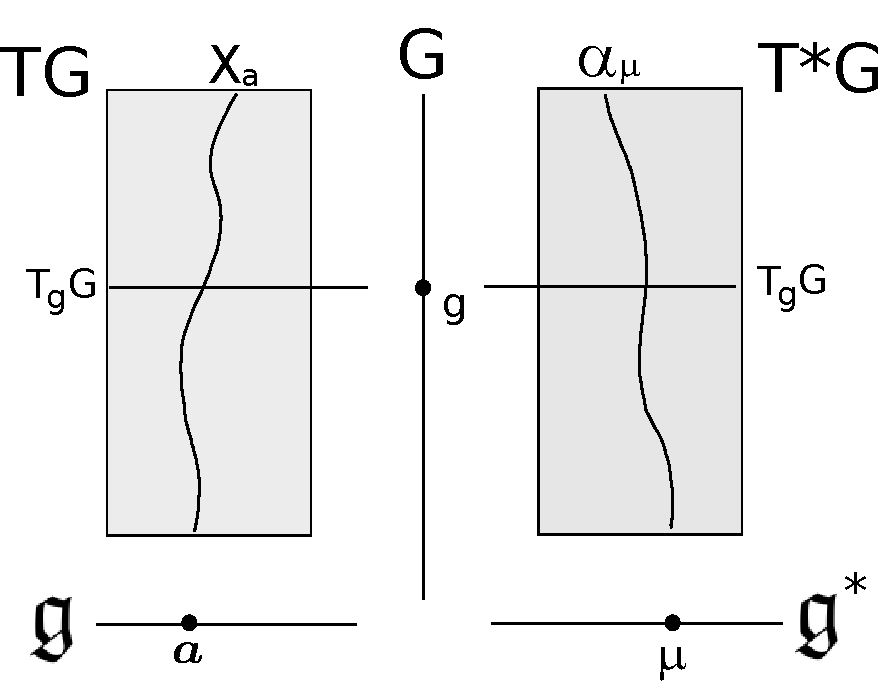
\includegraphics[width=10cm,keepaspectratio]{Fig/schemadoppiafibratura.pdf} \end{center} \end{frame}

\end{document}



